\section{Números de Precisão Finita}
\title{Aula 6 - Precisão Finita (parte 2)}
\begin{frame}
    \titlepage
\end{frame}

\begin{frame}{Complemento a 1}

    \begin{itemize}
        \item \textbf{Estratégia:} Inverter todos os bits para negar o número ($0 \rightarrow 1$ e $1 \rightarrow 0$).
        \item \textbf{Bit de Sinal:} O bit mais à esquerda define o sinal ($0$ pos, $1$ neg).



        \item Assim como no Sinal-Magnitude, o Complemento a 1 possui {\color{red}duas representações para o zero}:
              \begin{itemize}
                  \item \texttt{0000} ($+0$) e \texttt{1111} ($-0$ em $n=4$).
              \end{itemize}

        \item  \textbf{Antes do Complemento a 2, utilizava-se o Complemento a 1}

        \item  O \textbf{Complemento a 2} elimina o "zero duplo" e é o padrão nos computadores desde 1965.

    \end{itemize}
\end{frame}

\begin{frame}{Complemento a 1  com $n=4$}
    Observe como cada número negativo é exatamente a inversão bit a bit do seu equivalente positivo:

    \begin{center}
        \small
        \begin{tabular}{|c|c|c||c|c|}
            \hline
            \textbf{Decimal} & \textbf{Binário} & \textbf{Inversão}     & \textbf{Binário} & \textbf{Decimal} \\ \hline \hline
            $+0$             & \texttt{0000}    & $\longleftrightarrow$ & \texttt{1111}    & $-0$             \\ \hline
            $+1$             & \texttt{0001}    & $\longleftrightarrow$ & \texttt{1110}    & $-1$             \\ \hline
            $+2$             & \texttt{0010}    & $\longleftrightarrow$ & \texttt{1101}    & $-2$             \\ \hline
            $+3$             & \texttt{0011}    & $\longleftrightarrow$ & \texttt{1100}    & $-3$             \\ \hline
            $+4$             & \texttt{0100}    & $\longleftrightarrow$ & \texttt{1011}    & $-4$             \\ \hline
            $+5$             & \texttt{0101}    & $\longleftrightarrow$ & \texttt{1010}    & $-5$             \\ \hline
            $+6$             & \texttt{0110}    & $\longleftrightarrow$ & \texttt{1001}    & $-6$             \\ \hline
            $+7$             & \texttt{0111}    & $\longleftrightarrow$ & \texttt{1000}    & $-7$             \\ \hline
        \end{tabular}
    \end{center}

    \begin{itemize}
        \item \textbf{Funcionamento}: Para negar, basta aplicar o operador NOT (inverter 0 e 1).
        \item \textbf{O Problema:} Note o $+0$ (\texttt{0000}) e o $-0$ (\texttt{1111}). Essa duplicidade gera desperdício de uma combinação e circuitos de teste mais complexos.
    \end{itemize}
\end{frame}

\begin{frame}{Complemento a 2}
    Para encontrar o negativo de um número ($x \rightarrow -x$) em complemento a 2 faça o seguinte:

    \begin{enumerate}
        \item \textbf{Complemento a 1:} Inverta os bits.
        \item \textbf{Somar 1:} Adicione $1$ ao resultado obtido.
    \end{enumerate}

    \textbf{Exemplo de complemento a 2 ($+3 \rightarrow -3$):}
    \begin{itemize}
        \item $+3 = 0011_2$
        \item Inverte (complemento a 1 ) $\rightarrow 1100_2$
        \item Some $1 \rightarrow 1101_2$ (que é $-3$)
    \end{itemize}
\end{frame}

\begin{frame}{Complemento a 2: A Lógica dos Pesos}
    Neste sistema, o bit mais significativo (MSB) tem \textbf{peso negativo}, enquanto os demais mantêm pesos positivos:

    \begin{exampleblock}{Cálculo para $n=4$ bits}
        \begin{itemize}
            \item \texttt{0101} $= -0 \cdot 2^3 + 1 \cdot 2^2 + 0 \cdot 2^1 + 1 \cdot 2^0 = \mathbf{5}$
            \item \texttt{1011} $= -1 \cdot 2^3 + 0 \cdot 2^2 + 1 \cdot 2^1 + 1 \cdot 2^0 = -8 + 3 = \mathbf{-5}$
            \item \texttt{1111} $= -1 \cdot 2^3 + 1 \cdot 2^2 + 1 \cdot 2^1 + 1 \cdot 2^0 = -8 + 7 = \mathbf{-1}$
            \item \texttt{1000} $= -1 \cdot 2^3 + 0 + 0 + 0 = \mathbf{-8}$ \textit{(Mínimo)}
        \end{itemize}
    \end{exampleblock}

    \textbf{Vantagem:} O zero é único (\texttt{0000}) e as operações aritméticas são simplificadas no hardware.
\end{frame}



\begin{frame}{Tabela Completa: Complemento a 2 ($n=4$)}
    \begin{center}
        \small
        \begin{tabular}{|c|c||c|c|}
            \hline
            \textbf{Binário} & \textbf{Valor Decimal} & \textbf{Binário} & \textbf{Valor Decimal} \\ \hline \hline
            \texttt{0000}    & $0$                    & \texttt{1000}    & $-8$                   \\ \hline
            \texttt{0001}    & $+1$                   & \texttt{1001}    & $-7$                   \\ \hline
            \texttt{0010}    & $+2$                   & \texttt{1010}    & $-6$                   \\ \hline
            \texttt{0011}    & $+3$                   & \texttt{1011}    & $-5$                   \\ \hline
            \texttt{0100}    & $+4$                   & \texttt{1100}    & $-4$                   \\ \hline
            \texttt{0101}    & $+5$                   & \texttt{1101}    & $-3$                   \\ \hline
            \texttt{0110}    & $+6$                   & \texttt{1110}    & $-2$                   \\ \hline
            \texttt{0111}    & $+7$                   & \texttt{1111}    & $-1$                   \\ \hline
        \end{tabular}
    \end{center}
    \textbf{Faixa de Valores:} de $-2^{n-1}$ até $2^{n-1}-1$ (no caso, $-8$ a $+7$).
\end{frame}

\begin{frame}{Visualizacao circular Complemento a 2}
    \begin{center}
        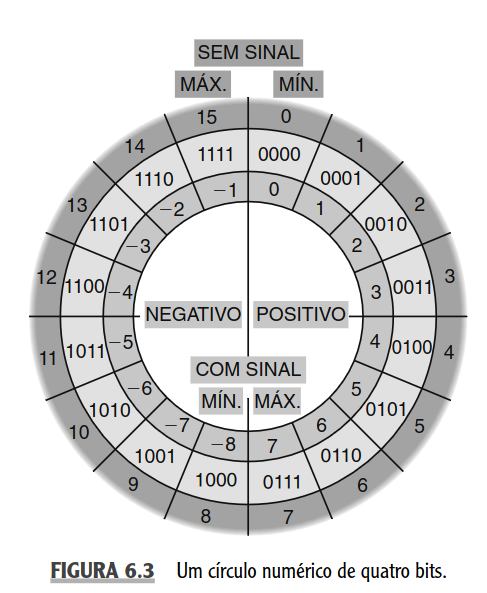
\includegraphics[width=0.5\textwidth]{Figuras/circulo-comp-a-2.png}

    \end{center}


\end{frame}

\begin{frame}{Números Positivos e o Zero em Complemento a 2}
    Para a faixa de $0$ até $2^{n-1}-1$, a representação em \textbf{Complemento a 2} é idêntica à de \textbf{Sinal-Magnitude}:

    \begin{block}{Regras de Representação}
        \begin{itemize}
            \item \textbf{Bit de Sinal:} O bit mais significativo (MSB) é sempre \textbf{0}.
            \item \textbf{Magnitude:} Os demais bits seguem a notação posicional binária padrão.
        \end{itemize}
    \end{block}



    \begin{exampleblock}{Exemplo ($n=4$)}
        O valor $+5_{10}$ é sempre \texttt{0101} em:
        \begin{itemize}
            \item Binário puro (4 bits)
            \item Sinal-Magnitude ($n=4$)
            \item Complemento a 2 ($n=4$)
        \end{itemize}
    \end{exampleblock}
\end{frame}
\begin{frame}{Números Negativos  em Complemento a 2}
    Para calcular a representação de um número negativo na faixa de $-1$ até $-2^{n-1}$, seguimos o algoritmo de três passos:

    \begin{alertblock}{Algoritmo de Conversão ($x \rightarrow -x$)}
        \begin{enumerate}
            \item \textbf{Magnitude:} Converte o valor absoluto do número para binário com $n$ bits.
            \item \textbf{Complemento a 1:} Inverte cada bit (0 vira 1, 1 vira 0).
            \item \textbf{Soma}  $1$ ao resultado anterior.
                  \begin{itemize}
                      \item \textit{Importante: Ignore o "vai-um" (carry-out) do bit mais significativo, se houver.}
                  \end{itemize}
        \end{enumerate}
    \end{alertblock}

    \textbf{Considere o descarte do carry}: Este processo garante que a soma de um número com seu negativo resulte em zero.
\end{frame}

\begin{frame}{Exemplos Práticos ($n=4$)}
    \begin{exampleblock}{Calculando o valor $-3$}
        \begin{itemize}
            \item \textbf{Passo 1 ($|3|$):} \texttt{0011}
            \item \textbf{Passo 2 (Comp. 1):} \texttt{1100}
            \item \textbf{Passo 3 (Soma 1):} \texttt{1100 + 1 = 1101}
            \item \textbf{Resultado:} $-3_{10} = 1101_2$
        \end{itemize}
    \end{exampleblock}

    \begin{exampleblock}{O caso do Zero ($0$)}
        \begin{itemize}
            \item \textbf{Passo 1 ($|0|$):} \texttt{0000}
            \item \textbf{Passo 2 (Comp. 1):} \texttt{1111}
            \item \textbf{Passo 3 (Soma 1):} \texttt{1111 + 1 = [1]0000}
            \item \textbf{Resultado:} \texttt{0000} (O "vai-um" é ignorado, mantendo o zero único).
        \end{itemize}
    \end{exampleblock}
\end{frame}

\begin{frame}{Resumo de Comparação ($n=4$)}
    Para o valor decimal \textbf{3}:

    \vspace{0.3cm}
    \begin{itemize}
        \item \textbf{Positivo ($+3$):} \texttt{0011}
        \item \textbf{Negativo ($-3$):} \texttt{1101}
    \end{itemize}

    \begin{center}
        \begin{tabular}{cr}
                        & \texttt{0011} ($+3$)            \\
            $+$         & \texttt{1101} ($-3$)            \\ \hline
            \small{[1]} & \texttt{0000} ($\phantom{[]}0$)
        \end{tabular}
    \end{center}

    \vspace{0.3cm}
    \textbf{Dica de Hardware:} Esse algoritmo é eficiente porque permite que o circuito de subtração seja basicamente um somador.
\end{frame}

\begin{frame}{Faixa de Representação em Complemento a 2}
    Para uma palavra de $n$ bits, a faixa de valores é assimétrica devido à representação única do zero:

    \begin{itemize}
        \item \textbf{Números Positivos e Zero:} De $0$ até $2^{n-1}-1$.
              \begin{itemize}
                  \item Temos $n-1$ bits disponíveis para a magnitude.
              \end{itemize}
        \item \textbf{Números Negativos:} De $-1$ até $-2^{n-1}$.
              \begin{itemize}
                  \item São $2^{n-1}$ combinações negativas.
              \end{itemize}
    \end{itemize}

    \begin{block}{Amplitude Total}
        A faixa completa vai de \textbf{$-2^{n-1}$ até $2^{n-1}-1$}.
        \begin{itemize}
            \item Total de valores: $2 \times 2^{n-1} = 2^n$ combinações distintas.
            \item \textbf{Vantagem:} Não há desperdício de combinação com o "zero duplo".
        \end{itemize}
    \end{block}
\end{frame}

\begin{frame}{Exercício: Complemento a 2 com $n=5$ bits}
    Escreva os números abaixo na base 2 usando a notação de \textbf{Complemento a 2}:

    \begin{enumerate}[a)]
        \item $-15$
        \item $-1$
        \item $0$
        \item $10$
    \end{enumerate}


\end{frame}

\begin{frame}{Respostas do Exercício ($n=5$)}
    Confira os resultados para a representação de 5 bits:

    \begin{table}[]
        \centering
        \begin{tabular}{|c|c|l|}
            \hline
            \textbf{Decimal} & \textbf{Binário (Complemento a 2)} & \textbf{Explicação}                                       \\ \hline
            $-15$            & \texttt{10001}                     & Inverte \texttt{01111} $\rightarrow$ \texttt{10000} $+ 1$ \\ \hline
            $-1$             & \texttt{11111}                     & Inverte \texttt{00001} $\rightarrow$ \texttt{11110} $+ 1$ \\ \hline
            $0$              & \texttt{00000}                     & Padrão único                                              \\ \hline
            $10$             & \texttt{01010}                     & Positivo direto                                           \\ \hline
        \end{tabular}
    \end{table}

    \vspace{0.4cm}
    \begin{description}
        \item[Dica para os negativos:]
              \begin{enumerate}
                  \item Ache o positivo em 5 bits (ex: $15 = 01111$).
                  \item Inverta os bits ($10000$).
                  \item Some 1 ($10001$).
              \end{enumerate}
    \end{description}

    \vspace{0.3cm}
    \textbf{Nota:} Em $n=5$, a faixa permitida é de $-16$ a $+15$. Todos os valores acima estão dentro do limite.
\end{frame}

\begin{frame}{Exercício: Interpretando Complemento a 2 ($n=7$)}
    Transcreva os números abaixo (em complemento a 2 de 7 bits) para a base 10.


    \begin{enumerate}[a)]
        \item \texttt{1111110}
        \item \texttt{1000001}
        \item \texttt{0111111}
        \item \texttt{1010101}
    \end{enumerate}


\end{frame}

\begin{frame}{Respostas do Exercício ($n=7$)}
    Confira os valores correspondentes na base 10:

    \begin{itemize}
        \item[\textbf{a)}] \texttt{1111110} $\rightarrow$ Inverte (\texttt{0000001}) $+ 1 = 0000010_2 \rightarrow \mathbf{-2}$
        \item[\textbf{b)}] \texttt{1000001} $\rightarrow$ Inverte (\texttt{0111110}) $+ 1 = 0111111_2 \rightarrow \mathbf{-63}$
        \item[\textbf{c)}] \texttt{0111111} $\rightarrow$ Começa com 0 (positivo) $\rightarrow 32+16+8+4+2+1 \rightarrow \mathbf{+63}$
        \item[\textbf{d)}] \texttt{1010101} $\rightarrow$ Inverte (\texttt{0101010}) $+ 1 = 0101011_2 \rightarrow \mathbf{-43}$
    \end{itemize}

    \textbf{Se a sequência começa com \textbf{1}, o número é negativo!}
\end{frame}

\begin{frame}{Negação (Inverso Aditivo) em Complemento a 2}
    "Negar" um número significa inverter o seu sinal ($x \rightarrow -x$).

    \begin{itemize}
        \item \textbf{No Sinal-Magnitude:} Basta inverter o bit mais significativo.
        \item \textbf{No Complemento a 2:} O processo de negação é \textbf{Complemento a 1 e Somar 1}.
    \end{itemize}

    \begin{block}{Algoritmo}
        Independentemente de o número original ser positivo ou negativo, o processo para encontrar seu inverso aditivo é o mesmo:
        \begin{enumerate}
            \item Inverte-se todos os bits ($0 \leftrightarrow 1$).
            \item Soma-se $1$ ao resultado.
        \end{enumerate}
    \end{block}

    \begin{exampleblock}{Exemplo ($n=4$): De $-3$ para $+3$}
        \begin{itemize}
            \item Partimos de $-3$: \texttt{1101}
            \item Invertemos os bits: \texttt{0010}
            \item Somamos $1$: \texttt{0010 + 1 = 0011} (que é $+3$)
        \end{itemize}
    \end{exampleblock}
\end{frame}

\begin{frame}{Exercício: Negação em 7 bits}
    Obtenha a representação da \textbf{negação} (inverso aditivo) de cada número abaixo, considerando a codificação Complemento a 2 com $n=7$:

    \begin{enumerate}[a)]
        \item \texttt{1111110}
        \item \texttt{1000001}
        \item \texttt{0111111}
        \item \texttt{1010101}
    \end{enumerate}

    \vspace{0.4cm}
    \textbf{Lembre-se:} O procedimento é o mesmo para todos: \textbf{Inverter + Somar 1}.
\end{frame}

\begin{frame}{Respostas: Inverso Aditivo ($n=7$)}
    \begin{itemize}
        \item[\textbf{a)}] \texttt{1111110} ($-2$)
              \begin{itemize}
                  \item Inverte (\texttt{0000001}) $+ 1 \rightarrow \mathbf{0000010}$ ($+2$)
              \end{itemize}
        \item[\textbf{b)}] \texttt{1000001} ($-63$)
              \begin{itemize}
                  \item Inverte (\texttt{0111110}) $+ 1 \rightarrow \mathbf{0111111}$ ($+63$)
              \end{itemize}
        \item[\textbf{c)}] \texttt{0111111} ($+63$)
              \begin{itemize}
                  \item Inverte (\texttt{1000000}) $+ 1 \rightarrow \mathbf{1000001}$ ($-63$)
              \end{itemize}
        \item[\textbf{d)}] \texttt{1010101} ($-43$)
              \begin{itemize}
                  \item Inverte (\texttt{0101010}) $+ 1 \rightarrow \mathbf{0101011}$ ($+43$)
              \end{itemize}
    \end{itemize}

    \begin{alertblock}{Atenção}
        A negação de um número positivo \textbf{sempre} resultará em um número começando com 1, e vice-versa (exceto para o zero).
    \end{alertblock}
\end{frame}

\begin{frame}{Adição em Complemento a 2}
    A grande vantagem do Complemento a 2 é que a adição é feita exatamente como nos números sem sinal, ignorando se o bit mais à esquerda representa sinal ou magnitude.

    \begin{block}{A Regra do Overflow}
        Diferente dos números sem sinal, o "vai-um" (carry-out) final não indica necessariamente um erro. No Complemento a 2, ocorre \textbf{overflow} apenas quando:
        \begin{itemize}
            \item Somamos dois números de \textbf{mesmo sinal} e o resultado tem \textbf{sinal oposto}.
        \end{itemize}
    \end{block}

    \begin{itemize}
        \item \textbf{Positivo + Negativo:} Nunca gera overflow.
        \item \textbf{Carry-out:} O vai-um que "sobra" à esquerda do bit de sinal deve ser \textbf{descartado}.
    \end{itemize}
\end{frame}

\begin{frame}{Exemplos de Adição ($n=8$)}
    \footnotesize
    \begin{columns}
        \begin{column}{0.5\textwidth}
            \textbf{1. Positivos (sem overflow):}
            \begin{center}
                \begin{tabular}{r@{\hspace{2pt}}c@{\hspace{2pt}}c@{\hspace{2pt}}c@{\hspace{2pt}}c@{\hspace{2pt}}c@{\hspace{2pt}}c@{\hspace{2pt}}c@{\hspace{2pt}}l}
                      &            &   & \color{red}1 & \color{red}1 &   & \color{red}1 & \color{red}1 &               \\
                      & \textbf{0} & 0 & 0            & 1            & 1 & 0            & 1            & $1_2$ ($27$)  \\
                    + & \textbf{0} & 1 & 0            & 0            & 1 & 0            & 0            & $1_2$ ($73$)  \\ \hline
                      & \textbf{0} & 1 & 1            & 0            & 0 & 1            & 0            & $0_2$ ($100$)
                \end{tabular}
            \end{center}

            \textbf{2. Negativos (sem overflow):}
            \begin{center}
                \begin{tabular}{r@{\hspace{2pt}}c@{\hspace{2pt}}c@{\hspace{2pt}}c@{\hspace{2pt}}c@{\hspace{2pt}}c@{\hspace{2pt}}c@{\hspace{2pt}}c@{\hspace{2pt}}l}
                    \color{red}1 & \color{red}1 & \color{red}1 & \color{red}1 & \color{red}1 &   & \color{red}1 & \color{red}1 &               \\
                                 & \textbf{1}   & 1            & 1            & 1            & 1 & 0            & 1            & $1_2$ ($-5$)  \\
                    +            & \textbf{1}   & 1            & 0            & 0            & 1 & 0            & 0            & $1_2$ ($-55$) \\ \hline
                    \small{[1]}  & \textbf{1}   & 1            & 0            & 0            & 0 & 1            & 0            & $0_2$ ($-60$)
                \end{tabular}
            \end{center}
        \end{column}
        \begin{column}{0.5\textwidth}
            \textbf{3. Sinais opostos:}
            \begin{center}
                \begin{tabular}{r@{\hspace{2pt}}c@{\hspace{2pt}}c@{\hspace{2pt}}c@{\hspace{2pt}}c@{\hspace{2pt}}c@{\hspace{2pt}}c@{\hspace{2pt}}c@{\hspace{2pt}}l}
                      &            &   & \color{red}1 & \color{red}1 &   & \color{red}1 & \color{red}1 &               \\
                      & \textbf{1} & 1 & 0            & 0            & 1 & 0            & 0            & $1_2$ ($-55$) \\
                    + & \textbf{0} & 0 & 0            & 1            & 1 & 0            & 1            & $1_2$ ($27$)  \\ \hline
                      & \textbf{1} & 1 & 1            & 0            & 0 & 1            & 0            & $0_2$ ($-28$)
                \end{tabular}
            \end{center}

            \textbf{4. Negativos com Overflow:}
            \begin{center}
                \begin{tabular}{r@{\hspace{2pt}}c@{\hspace{2pt}}c@{\hspace{2pt}}c@{\hspace{2pt}}c@{\hspace{2pt}}c@{\hspace{2pt}}c@{\hspace{2pt}}c@{\hspace{2pt}}l}
                    \color{red}1 &            &   & \color{red}1 & \color{red}1 &   & \color{red}1 & \color{red}1 &                   \\
                                 & \textbf{1} & 0 & 0            & 1            & 1 & 0            & 1            & $1_2$ ($-99$)     \\
                    +            & \textbf{1} & 1 & 0            & 0            & 1 & 0            & 0            & $1_2$ ($-60$)     \\ \hline
                    \small{[1]}  & \textbf{0} & 1 & 1            & 0            & 0 & 1            & 0            & $0_2$ \textbf{!!}
                \end{tabular}
            \end{center}
            \textit{Erro: Negativo + Negativo deu Positivo.}
        \end{column}
    \end{columns}
\end{frame}

\begin{frame}{Subtração em Complemento a 2}
    A subtração é simplificada transformando-a em uma adição com o inverso aditivo:

    \begin{center}
        \Large $A - B \implies A + (-B)$
    \end{center}

    \begin{block}{Procedimento}
        \begin{enumerate}
            \item Mantenha o primeiro operando ($op1$).
            \item Calcule o \textbf{Complemento a 2} do segundo operando ($op2$).
            \item Some os dois valores seguindo as regras da adição.
        \end{enumerate}
    \end{block}
    Isso permite que o hardware use o mesmo circuito somador para as duas operações.
\end{frame}

\begin{frame}{Exercício: Aritmética com 4 bits}
    Realize as operações usando \textbf{Complemento a 2 com 4 bits}. Indique se houve overflow.

    \begin{columns}
        \begin{column}{0.5\textwidth}
            \begin{enumerate}[a)]
                \item $5 - 3$
                \item $2 - 4$
                \item $(-5) + (-1)$
            \end{enumerate}
        \end{column}
        \begin{column}{0.5\textwidth}
            \begin{enumerate}[d)]
                \setcounter{enumi}{3}
                \item $4 + 2$
                \item $7 + 3$
                \item $(-4) + (-5)$
            \end{enumerate}
        \end{column}
    \end{columns}

    \vspace{0.5cm}
    \textbf{Lembre-se da faixa de 4 bits:} $[-8, +7]$.
\end{frame}

\begin{frame}{Gabarito: Aritmética com 4 bits}
    \footnotesize
    \begin{itemize}
        \item[\textbf{a)}] $0101 + 1101 = [1]0010$ ($+2$) \hfill \textbf{OK}
        \item[\textbf{b)}] $0010 + 1100 = 1110$ ($-2$) \hfill \textbf{OK}
        \item[\textbf{c)}] $1011 + 1111 = [1]1010$ ($-6$) \hfill \textbf{OK}
        \item[\textbf{d)}] $0100 + 0010 = 0110$ ($+6$) \hfill \textbf{OK}
        \item[\textbf{e)}] $0111 + 0011 = \mathbf{1010}$ \hfill \textbf{OVERFLOW!}
              \begin{itemize}
                  \item \textit{Positivo + Positivo resultou em negativo.}
              \end{itemize}
        \item[\textbf{f)}] $1100 + 1011 = [1]\mathbf{0111}$ \hfill \textbf{OVERFLOW!}
              \begin{itemize}
                  \item \textit{Negativo + Negativo resultou em positivo.}
              \end{itemize}
    \end{itemize}
\end{frame}

\begin{frame}{Multiplicação e Divisão em Complemento a 2}
    Diferente da adição, a multiplicação e a divisão no Complemento a 2 geralmente seguem uma estratégia de "valor absoluto":

    \begin{block}{Algoritmo Geral}
        \begin{enumerate}
            \item \textbf{Preparação:} Se um operando for negativo, calcula-se seu Complemento a 2 para obter o valor absoluto ($|x|$).
            \item \textbf{Operação:} Multiplica-se ou divide-se os valores absolutos como números sem sinal.
            \item \textbf{Sinal do Resultado:}
                  \begin{itemize}
                      \item Sinais iguais $\rightarrow$ Resultado Positivo.
                      \item Sinais opostos $\rightarrow$ Calcula-se o Complemento a 2 do resultado para torná-lo negativo.
                  \end{itemize}
        \end{enumerate}
    \end{block}

    \begin{alertblock}{Overflow na Multiplicação}
        Em uma representação de $n$ bits, ocorre overflow se o produto dos valores absolutos atingir o bit de sinal ($n-1$) ou além.
    \end{alertblock}
\end{frame}

\begin{frame}{Exemplos de Multiplicação ($n=8$)}
    \footnotesize
    \textbf{1. Positivos com Overflow:} $27 \times 5 = 135$ (Limite é $127$)
    \begin{tabular}{ccccccccc}
                 & {\bf 0}                         & 0                             & 0                             & 1                             & 1 & 0 & 1 & $1_2$ \\
        $\times$ & {\bf 0}                         & 0                             & 0                             & 0                             & 0 & 1 & 0 & $1_2$ \\
        \hline
                 & {\footnotesize  \color{red}1}!! & {\footnotesize  \color{red}1} & {\footnotesize  \color{red}1} & {\footnotesize  \color{red}1} &   &   &   &       \\
                 & {\bf 0}                         & 0                             & 0                             & 1                             & 1 & 0 & 1 & 1     \\
        +        & {\bf 0}                         & 1                             & 1                             & 0                             & 1 & 1 &   &       \\
        \hline
                 & {\bf 1}!!                       & 0                             & 0                             & 0                             & 0 & 1 & 1 & 1     \\
        \\
    \end{tabular}

    \textbf{2. Positivos sem Overflow:} $11 \times 5 = 55$

    \begin{tabular}{ccccccccc}
                 & {\bf 0} & 0 & 0 & 0                             & 1 & 0 & 1 & $1_2$ \\
        $\times$ & {\bf 0} & 0 & 0 & 0                             & 0 & 1 & 0 & $1_2$ \\
        \hline
                 &         &   &   & {\footnotesize  \color{red}1} &   &   &   &       \\
                 & {\bf 0} & 0 & 0 & 0                             & 1 & 0 & 1 & 1     \\
        +        & {\bf 0} & 0 & 1 & 0                             & 1 & 1 &   &       \\
        \hline
                 & {\bf 0} & 0 & 1 & 1                             & 0 & 1 & 1 & 1     \\
        \\
    \end{tabular}
\end{frame}


\begin{frame}{Exemplo: Multip. de positivo e um negativo com {\em overflow}}
    Considere: ${\bf 1}0001011_2$ ($-117$) $\times$ ${\bf 0}0000101_2$ ($5$) em $n=8$.


    \textbf{Passo 1: Obter valor absoluto de $-117$:}

    \begin{tabular}{ccccccccc}
            & {\bf 1} & 0 & 0 & 0 & 1 & 0 & 1 & $1_2$ \\
        \hline
        inv & {\bf 0} & 1 & 1 & 1 & 0 & 1 & 0 & $0_2$ \\
        +   &         &   &   &   &   &   &   & 1     \\
        \hline
            & {\bf 0} & 1 & 1 & 1 & 0 & 1 & 0 & $1_2$ \\
        \\
    \end{tabular}

    \textbf{Passo 2: Multiplicar $117 \times 5$:}
    \begin{tabular}{ccccccccc}
                                      & {\bf 0}                       & 1                             & 1                             & 1 & 0                             & 1 & 0 & $1_2$ \\
        $\times$                      & {\bf 0}                       & 0                             & 0                             & 0 & 0                             & 1 & 0 & $1_2$ \\
        \hline
        {\footnotesize  \color{red}1} & {\footnotesize  \color{red}1} & {\footnotesize  \color{red}1} & {\footnotesize  \color{red}1} &   & {\footnotesize  \color{red}1} &   &   &       \\
                                      & {\bf 0}                       & 1                             & 1                             & 1 & 0                             & 1 & 0 & 1     \\
        + {\bf 1}!!                   & {\bf 1}!!                     & 1                             & 0                             & 1 & 0                             & 1 &   &       \\

        \hline
        ... !!                        & {\bf 0}                       & 1                             & 0                             & 0 & 1                             & 0 & 0 & 1     \\
    \end{tabular}


\end{frame}

\begin{frame}{Expansão de Bits (Extensão de Sinal)}
    Frequentemente, precisamos converter um número de $n$ bits para uma representação de $m$ bits ($m > n$) mantendo seu valor original.

    \begin{block}{A Regra da Extensão de Sinal}
        Para expandir um número em \textbf{Complemento a 2}:
        \begin{enumerate}
            \item Move-se o bit de sinal para a nova posição mais à esquerda.
            \item Preenchem-se as novas posições com o \textbf{mesmo valor do bit de sinal}.
        \end{enumerate}
    \end{block}

    \begin{itemize}
        \item Se o número é \textbf{positivo} (MSB=0), preenchemos com \textbf{0}s à esquerda.
        \item Se o número é \textbf{negativo} (MSB=1), preenchemos com \textbf{1}s à esquerda.
    \end{itemize}
\end{frame}

\begin{frame}{Exemplos de Expansão ($4 \rightarrow 8$ bits)}
    \begin{exampleblock}{Exemplo 1: Valor Positivo ($+4$)}
        \begin{itemize}
            \item Representação 4 bits: {\color{blue}0}100
            \item Extensão para 8 bits: {\color{blue}0000}{\color{blue}0}100
        \end{itemize}
    \end{exampleblock}

    \begin{exampleblock}{Exemplo 2: Valor Negativo ($-4$)}
        \begin{itemize}
            \item Representação 4 bits: {\color{red}1}100
            \item Extensão para 8 bits: {\color{red}1111}{\color{red}1}100
        \end{itemize}
    \end{exampleblock}

    \vspace{0.3cm}
    \textbf{Por que funciona?}
    No caso do $-4$:
    \begin{itemize}
        \item 4 bits: $-8 + 4 = -4$
        \item 8 bits: $-128 + 64 + 32 + 16 + 8 + 4 = -128 + 124 = -4$
    \end{itemize}
\end{frame}
\begin{frame}{Exercício: Extensão de Sinal e Hexadecimal}
    Mostre que os valores hexadecimais abaixo, em notação de \textbf{Complemento a 2}, representam o valor $-5_{10}$:

    \begin{enumerate}[a)]
        \item \texttt{B} ($n=4$ bits)
        \item \texttt{FB} ($n=8$ bits)
        \item \texttt{FFB} ($n=12$ bits)
    \end{enumerate}

    \begin{block}{Dica de Resolução}
        Converta o dígito mais significativo para binário e verifique o bit de sinal.
        \begin{itemize}
            \item \texttt{B} em binário é \texttt{1011}.
            \item Como o MSB é \textbf{1}, o número é negativo.
            \item Aplique o processo inverso (Inverter + Somar 1) para conferir a magnitude.
        \end{itemize}
    \end{block}
\end{frame}

\begin{frame}{Resolução: A consistência do $-5$}
    \small
    \begin{itemize}
        \item[\textbf{a)}] \texttt{B} $\rightarrow$ \texttt{1011}.
              \begin{itemize}
                  \item Inverso: \texttt{0100 + 1 = 0101} ($5_{10}$). Logo: \textbf{$-5$}.
              \end{itemize}
        \item[\textbf{b)}] \texttt{FB} $\rightarrow$ \texttt{1111 1011}.
              \begin{itemize}
                  \item Inverso: \texttt{0000 0100 + 1 = 0000 0101} ($5_{10}$). Logo: \textbf{$-5$}.
              \end{itemize}
        \item[\textbf{c)}] \texttt{FFB} $\rightarrow$ \texttt{1111 1111 1011}.
              \begin{itemize}
                  \item Inverso: \texttt{0000 0000 0100 + 1 = 0000 0101} ($5_{10}$). Logo: \textbf{$-5$}.
              \end{itemize}
    \end{itemize}

    \begin{alertblock}{Conclusão}
        Note que \texttt{FB} e \texttt{FFB} são apenas extensões de sinal de \texttt{B}. Em hexadecimal, se o número for negativo, ele será preenchido com \texttt{F} ($1111_2$) à esquerda.
    \end{alertblock}
\end{frame}

\begin{frame}{Redução e Truncamento}
    O caminho inverso (reduzir o número de bits) nem sempre preserva o valor. Ao truncar de $n$ para $k$ bits ($k < n$), eliminamos os $n-k$ bits mais significativos.

    \begin{itemize}
        \item \textbf{Números sem sinal:} O truncamento equivale a $x \bmod 2^k$.
    \end{itemize}

    \begin{exampleblock}{Exemplo: Truncando $1100_2$ ($12_{10}$)}
        \begin{itemize}
            \item \textbf{Para 3 bits:} $1|100 \rightarrow 100_2$ ($4_{10}$).
                  \begin{itemize}
                      \item Cálculo: $12 \bmod 2^3 = 12 \bmod 8 = 4$.
                  \end{itemize}
            \item \textbf{Para 2 bits:} $11|00 \rightarrow 00_2$ ($0_{10}$).
                  \begin{itemize}
                      \item Cálculo: $12 \bmod 2^2 = 12 \bmod 4 = 0$.
                  \end{itemize}
        \end{itemize}
    \end{exampleblock}

    \textbf{Atenção:} No Complemento a 2, o truncamento pode alterar drasticamente o valor e até o \textbf{sinal} do número!
\end{frame}


